\newpage
\chapter{Similar-sized collisions: A parameter study}
\graphicspath{{./03figs/}}

A collision is cratering, when the impactor is much smaller than the target. In this case, the impactor hits the target completely and comes to a full stop, the result is a crater. Such a collision corresponds to a point source energy input into the target and can be treated like an explosion \citep{Melosh:2007p3502}. Scaling laws exist for the resulting crater depth and shape \citep{Holsapple:1993p3018}. 

In cratering collisions the impactor partly misses the target only for very grazing impact angles $\thimp \approx 90 \deg$ and the result deviates from pure cratering and becomes none-trivial. Such a case is shown in figure \label{ch03_fig03} on the right side where $\Rimp \ll \Rtar$. So a cratering collision results either in a complete hit or a complete miss. If on the other hand the target and the impactor are similar in size, this critical angle becomes much smaller than $90 \deg$ and the collision is called similar-sized, this is depicted on the left side of the figure in which case $\theta_{graz} \approx 45^\circ$. This grazing angle where roughly half of the impactor misses the target yields
\begin{equation}
\label{ch03_eq001}
\cos{ \theta_{graz} }= \frac{\Rtar}{\Rtar + \Rimp}
\end{equation}

\begin{figure}[htbp]
\begin{center}
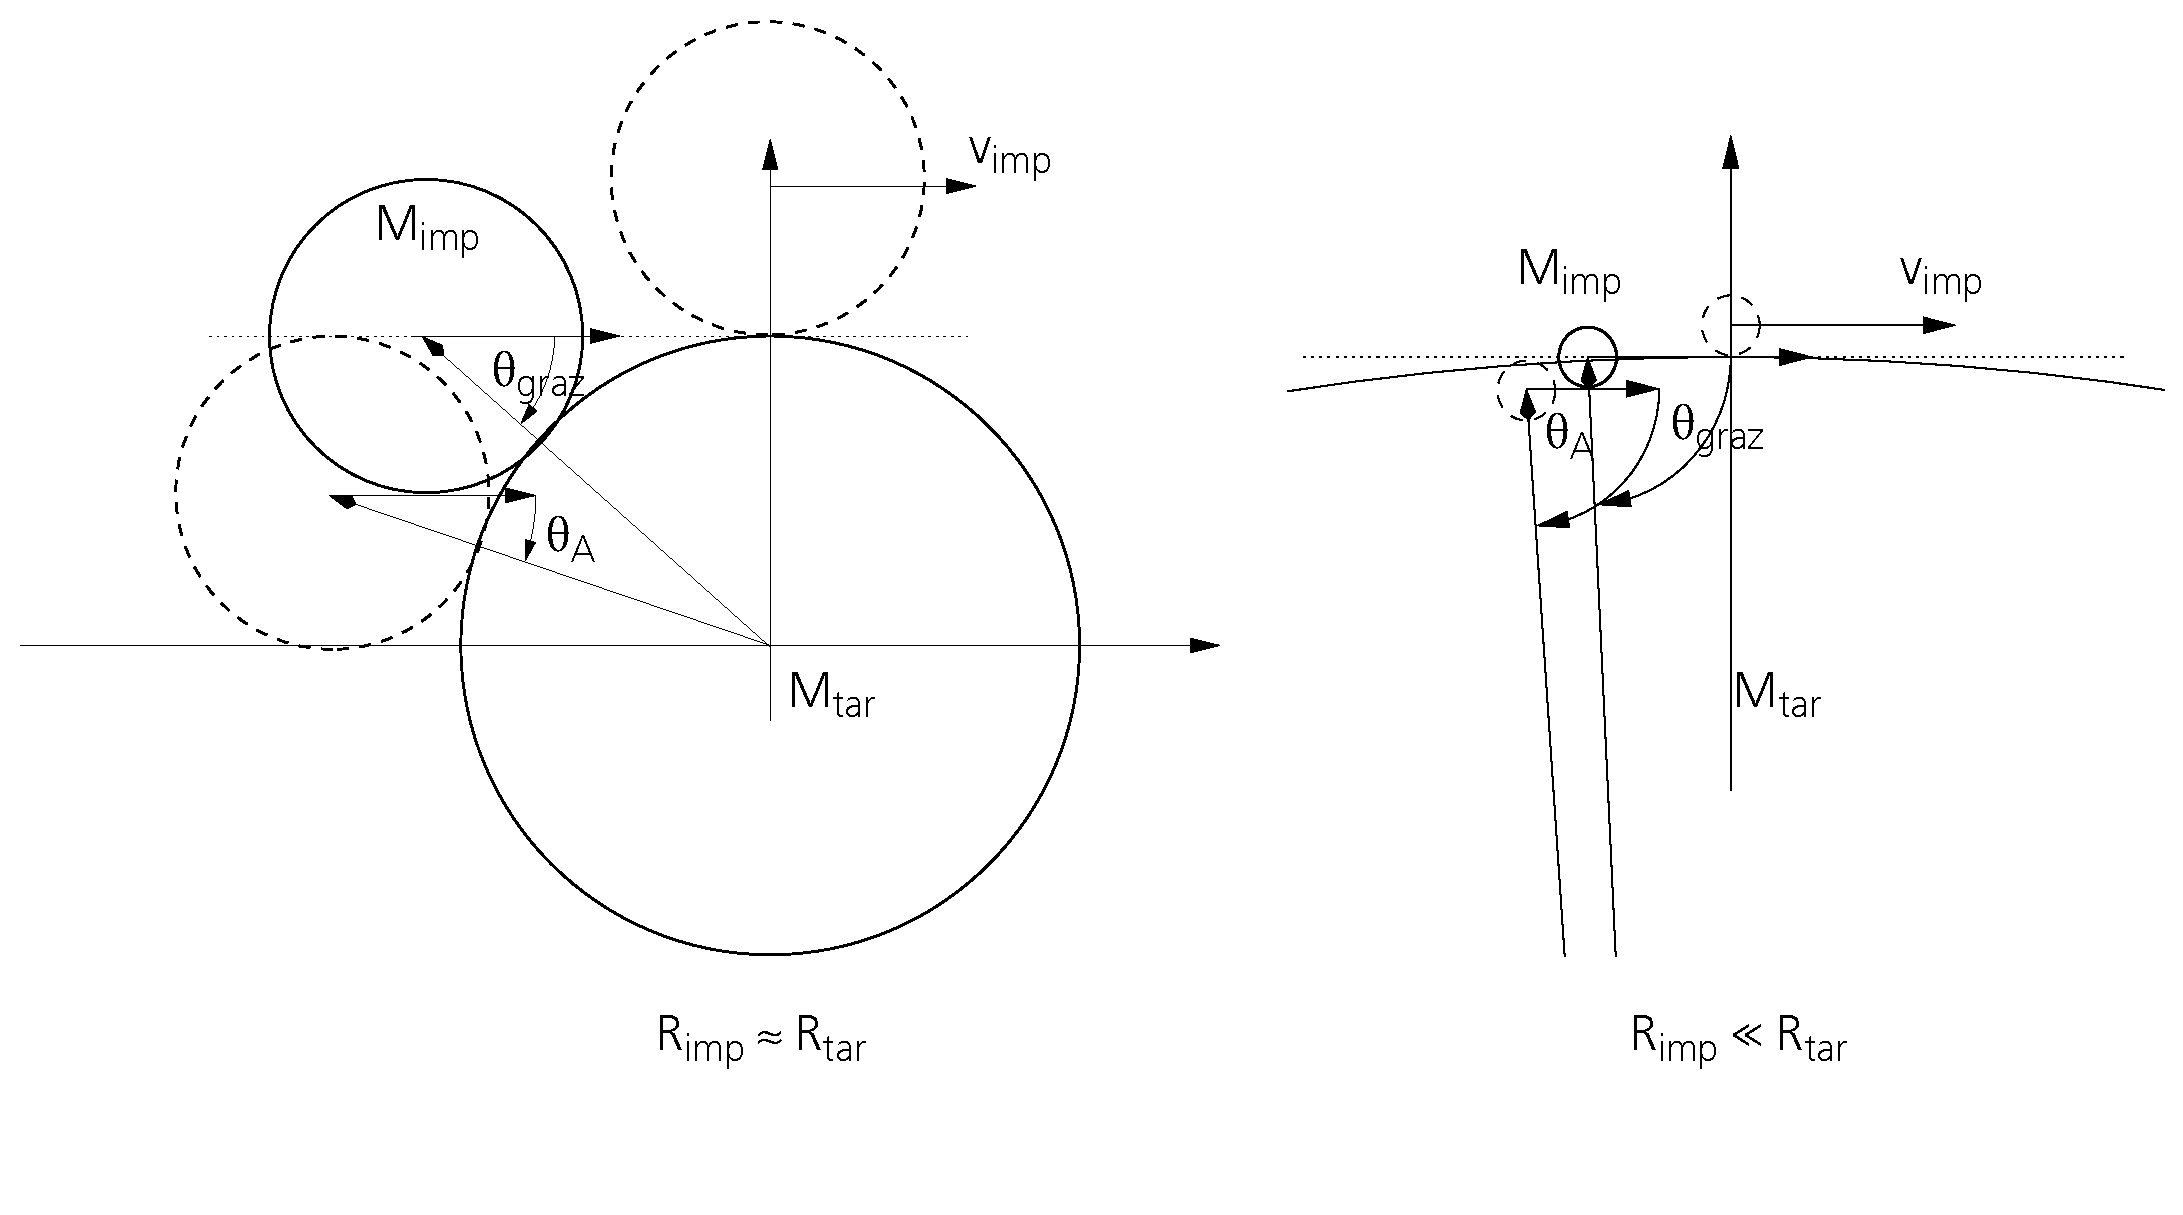
\includegraphics[scale=0.4]{03_grazing}
\caption{Impact geometry for a \SSC on the left side. The right plot shows a collision between a relatively small impactor compared to the target. The grazing impact angle $\theta_{graz}$ is defined as the angle for which half of the impactor simply grazes past the target \citep{Asphaug:2010p3539}. The dashed circles show the largest impact angle for which no impactor material would graze past the target $\theta_A$ and the $90^\circ$ impact angle for which the whole impactor grazes past the target.}
\label{ch03_fig03}
\end{center}
\end{figure}

\begin{figure}[htbp]
\begin{center}
\includegraphics[scale=0.7]{05_Mhit}
\caption{Relative volume of the impactor ($V_{hit, imp}$, left plots) and the target ($V_{hit, tar}$, right plots) hit by the other body as a function of impact angle (top plots) and impact parameter (bottom plots) for different mass ratios $\gamma$. Compare figure \ref{ch07_fig01} for an illustration of those volumes. Note that the ratio of radii scales with the cubic root of the mass ratio: $R_{imp} / R_{tar} \sim \sqrt[3]{\gamma}$. The dotted line shows for which impact angle half of the impactor volume grazes past the target. } 
\label{ch03_fig05}
\end{center}
\end{figure}

Assuming the impactor follows a straight trajectory, the volume missing the target can be calculated by integrating the cross section along the target volume (Compare appendix \ref{ch07_sec01} for the derivation). Figure \ref{ch03_fig05} on the left side shows the relative volume of the impactor missing the target ($V_{hit, imp}$) as a function of impact angle for different mass ratios $\gamma$ assuming constant and equal density spheres as bodies. The volume follows a step-function for very small impactors (small $\gamma$) with a sharp drop-off to zero near $90 \deg$. For similar-sized collisions with $\gamma = 0.1 \dots 1.0$ the relative volume smoothly increases for smaller impact angles opens the possibility for a variety of collisional outcomes between a total hit and a total miss. For example even for a rather small $\gamma = 0.1$, the relative volume hit by the impactor varies between 0 and 1 over an impact angle range of $30 \deg$.

Similar sized collisions are interesting, because bodies in planetary systems grow mainly by big accretionary events. Or in other words, the evolution of the largest bodies is dominated by similar-sized collisions. Many phenomena in planetary systems can best be explained as direct results of similar-sized collisions. Examples are the formation of the Earths Moon \citep{Benz:1985p1755}, Plutos companion Charon \cite{Canup:2005p1987} or also the anomalously high density of Mercury \cite{Benz:1988p3336}. Understanding similar-sized collisions is therefore key for understanding planet formation in general.

Compared to cratering collisions the interplay of the governing physics is more complex and there are only very basic scaling laws predicting the outcomes of similar-sized collisions. Hydrodynamics, gravity and thermodynamics interact in a interacted way and need to be simulated explicitly. The goal of this chapter is to perform a small parameter study in the regime of similar-sized collisions by performing a large number of impact simulations and then looking at various characteristic parameters describing the outcome of the collisions. The first section gives a quick overview of the physical processes involved in similar sized collisions and their associated timescales. In a second section, the detailed setup of the simulations and the used parameters are described. The actual results are presented in the third and discussed in the fourth section.

\section{Physics of similar-sized collisions}
Looking at the associated timescales of physics gives a feeling on what are the important aspect of physics in similar-sized collisions. In the gravity regime, where the impact velocities are in the order of the mutual escape velocity, similar-sized collisions possess the nice property scale-invariance on the first order: When the impact velocity is scaled to the escape velocity $\vesc$ and time to the collisional time $\tcol = ( \Rimp + \Rtar ) / \vesc$ the collision becomes self-similar. In other words: A collision at a given impact velocity and angle for a certain mass ration $\gamma = \Mimp / \Mtar$ has the same outcome for a target mass of $0.01 \ME$ and $1.0 \ME$ assuming the bodies have in both cases the same density and effects like shocks or compressibility can be neglected.

The collisional timescale is an estimate on how long it takes for the impactor to penetrate into the target and is given by
\begin{align}
\tau_{coll} = \frac{2 (\Rimp + \Rtar)}{\vimp} \sim \frac{\vesc}{\vimp} \frac{2 R_{tot}}{\vesc} \sim \frac{\vesc}{\vimp}  \frac{2 R_{tot}}{\sqrt{G \rho} R_{tot}} \sim \frac{\vesc}{\vimp} \frac{1}{\sqrt{\rho}}
\end{align}
where the mutual escape velocity is given by $\vesc = \sqrt{ 2 G \frac{\Mtar + \Mimp}{\Rtar + \Rimp} }$ and constant density bodies are assumed. Gravitational restitution happens on the gravitational timescale given by
\begin{align}
\tau_{grav} = \sqrt{\frac{3 \pi }{G \rho} } \sim \frac{1}{\sqrt{\rho}}
\end{align}
and is in the same order of magnitude as the collisional timescale. Both timescales depend on the bodies density. The collisional timescale also weakly depends on the mass ratio ($\sim \sqrt[3]{\gamma}$), but stays still in the same order of magnitude for the similar sized collisions mass ratios of $\gamma = 0.1 \dots 1$. For a collisions between with $\Mimp = \Mtar = 0.1\ME$ and $\Rimp = \Rtar = 0.55 \RE$ at their mutual escape velocity, the collisional timescale yields $50$ min, whilst the gravitational timescale for a mean-density of $4g/cm^3$ is around $100$ mins. 

Other physical effects are not scale-invariant, for example viscosity. \cite{Asphaug:2010p3539} argues as follows, that viscosity can be neglected in similar-sized collisions for bodies of at least a certain size: Characteristic stresses due to gravity are 
\begin{equation}
\sigma_{grav} \sim P_0 \sim G \rho^2 R^2
\end{equation}
where $P_0$ is the pressure inside the body with radius $R$. The strain rate $\dot{\epsilon}$ for a given Newtonian viscosity $\nu$ is then
\begin{equation}
\dot{\epsilon} = \frac{\sigma}{\nu}
\end{equation}
The strain which can develop over a gravitational timescale under viscosity is then
\begin{equation}
\epsilon = \frac{\dot{\epsilon}}{\tau_{grav}}
\end{equation}
Viscosity becomes an important effect, if the maximal strain which can develop over a gravitational timescale is only around unity. Or in other words, when the timescale for a strain of around unity becomes the same order of magnitude as the gravitational timescale, then viscosity is an important effect. Viscosity in the mantle of the early Earth was around $\nu \approx 10^9~\textrm{poise}$ \citep{2004Tectp.384...55W}, whereas for completely molten rock even lower values of around $\nu \approx 10^8~\textrm{poise}$ expected. \cite{Asphaug:2010p3539} gives a lower limit of a few $100km$ for solid and around $10km$ for partially molten bodies for which viscosity can be neglected and using a inviscid hydrodynamics solver is valid. Large bodies can be assumed to be molten during the early stages of planet formation 

Shocks are another effects where similar-sized collisions deviate from scale-invariance: The escape velocity scales $\vesc \sim M^\frac{1}{3}$ for constant density bodies \footnote{$\vesc = \sqrt[6]{8 \pi G^3 \rho} M^\frac{1}{3} \sim M^\frac{1}{3}$} and is around $1km/s$ for a density of $4g/cm^3$ and a mass of $10^{-3} \ME$. This is below the speed of sound in silicates ($\approx 3 km/s$, \cite{Melosh:2007p3502}), so that a collision with an impact velocity on the order of the escape velocity will produce acoustic waves but no strong shocks. For bodies with masses higher than a few Moon masses, the impact velocity comes into the same range as the speed of sound. Collisions now are in the hypervelocity regime and produce strong shock, leading to a considerable heating. 

The goal of this parameter study is now to get quantitative results for various quantities and to check whether they are scale-invariant or not.


\section{Setup and parameters used}
A similar-sized collisions encompasses many parameters, the most important ones being target mass $\Mtar$, impactor mass $\Mimp$, impact velocity $\vimp$ and impact angle $\thimp$. Often the scaled impact parameter $b'=\sin{\thimp}$ is used instead of the impact angle. These parameters span a 4-dimensional parameter space which will be explored in this parameter study. 

Additional parameters are the pre-impact rotation of both the impactor and the target, which in principle spans another 6-dimensions into the parameter space. Another parameter study concerning the formation of the Earths Moon by \cite{Canup:2008p3551} analyzed the effect of pre-impact rotation of the two bodies onto disk formation after the collision and found it to be non-negligible. The composition and interior thermal profiles of both bodies are also inform parameters. They both determine the density distribution inside the bodies and therefore also the dynamics of the collision. The internal profile furthermore determines the radius of the body and therefore the impact geometry, the mutual escape velocity and accordingly the actual impact velocity. These additional parameters are not further explored in this study.

\begin{figure}[htbp]
\begin{center}
\includegraphics[scale=0.7]{01_overview_params.pdf}
\caption{Overview of the sampling points in the 4-dimensional parameter space spanned by $\big\{ \Mtar, \Mimp, \thimp, \vimp / \vesc \big\}$. The left plot shows the mass pairs for both bodies. Grey points denote \emph{r3} bodies (pure silicate), red points \emph{c1} bodies (chondritic, differentiated) and blue points \emph{i1} bodies (icy, differentiated). For each mass pair a total of 105 simulations sample the $\big\{ \thimp, \vimp / \vesc \big\}$ sub-space. Points in this sub-space are }
\label{ch03_fig01}
\end{center}
\end{figure}
\begin{figure}[htbp]
\begin{center}
\includegraphics[scale=0.8]{07_strucs.pdf}
\caption{Isentropic internal structures of the bodies used in the simulations. The first row of plots shows the density profiles, the second row the pressure and the third row the temperatures. The first column of plots shows silicate bodies with a $100 wt\%$ $\silc$ composition with the following masses from left to right: 0.1 (blue curve), 0.2 (red), 0.5 $\ME$ (magenta). The second column shows structures of differentiated bodies of chondritic composition with a $70 wt\%$ $\silc$ mantle and a $30 wt\%$ iron core: 0.002 (red), 0.007 (green), 0.01 (blue), 0.02 (red), 0.035 (black), 0.07 (green), 0.1 (blue), 0.2 (red), 0.7 (green) and 1.0 $\ME$ (blue). The last column on the right shows a few structures with a composition typical to regions beyond the snow line with $50 wt\%$ water ice, $35 wt\%$ $\silc$ and $15 wt\%$ iron. Masses range from 0.002 (red), 0.01 (blue), 0.02 (red), 0.1 (blue), 0.2 (red) and 1.0 $\ME$ (blue) from left to right. The radius of the structures depends on the average density and therefore also on the composition of the bodies. Icy bodies have low average densities compared to chondritic bodies. Note that the bodies entirely composed of $\silc$ have a higher average density than equally massive bodies with a chondritic composition, due to the higher compressibility of $\silc$ compared to iron. In the core of the pure silicate bodies, the density reached more than twice the reference density of $\silc$, while the iron cores of the chondritic bodies is only slightly compressed.}
\label{ch03_fig07}
\end{center}
\end{figure}

The strategy for sampling the parameter space goes as follows: For three different types of body composition sets of simulations are performed. Simulation set \emph{r3} uses homogeneous bodies made up of $100 \wtp~\silc$, simulation set \emph{c1} differentiated bodies with a chondritic composition of $70 \wtp~\silc$ and $30 \wtp~\iron$ and simulation set \emph{i1} uses differentiated bodies with a composition typical beyond the snow line of of $50 \wtp~\watr$, $35 \wtp~\silc$ and $15 \wtp~\iron$. Figure \ref{ch03_fig07} shows the internal structures for this three different types of bodies.

Target masses 

% TODOPLOT: show config matrix with all the parameters used (initial temperature, nop, mass)
describe parameter space: fixed target mass and mass ratio, then vary relative impact velocity and impact angle. hit\&run are not considered. \\
how long a simulation is integrated \\
problems: timescales too long\\
post-processing \\
r3, c1, i1 \\
resolution, number of particles, particles per body diameter \\
initial temperature not important, show profiles nevertheless \\
give an overview of the result parameters\\

how to setup
as shown in \ref{ch02_sec04_ss02} and \label{ch02_sec04_ss04}





\section{Results}
%%
% Largest remnant
%% 
\subsection{Largest remnant mass, accretion efficiency $\xi$ and $Q_D$}
compare with previous work\\
\cite{Benz:1988p3336} 0.1 Mearth target, 1:6 mass ratio, vimp = 2.5-8 vesc, all eroding\\
\cite{Benz1999Icar..142....5B}: MLR / Mtarg ~ Q / Q*, parabolic fit \\
\cite{Agnor:2004p3329}  two 0.1Mearth mass bodies, chondritic, Tillotson \\
\cite{Stewart:2009p3265} catastrophic disruption criteria, Mlr / Mtarg replaced by Mlr / Mtot, Q* scaled to reduced mass in kinetic energy \\ 
\cite{2010ApJ...714L..21K} ,mass ratios: 1.0, 0.66, 0.50, 0.33, 0.25, 0.17, 0.11, Mtot = 0.2-2.0MEarth, defined $v_{cr}$ \\
try volumetric scaling for oblique impacts \\
show 4 main categories: accretion, partial accretion, erosion and hit \& run \\
check Benz 1999, Angor \& Asphaug 2004, Stewart \& Leinhardt 2009, Marcus 2009, Marcus 2010 \\
volumetric scaling (Canup 2005, Leinhardt) \\
mention problems with slow accretion producing secondary impacts, show example with very large timescales, problem to estimate result due to pre-rotation\\

\begin{landscape}
\begin{figure}[htbp]
\begin{center}
\includegraphics[scale=1.0]{08_accreff_r3.pdf}
\caption{Accretion efficiency $\xi$ as a function of the impact angle for different relative impact velocities. Each subplot shows a set of simulations for a given target mass $\Mtar$ and mass ratio $\gamma = \Mimp / \Mtar$. Each point shows the outcome of an individual simulation of the \emph{r3} simulation set involving bodies composed purely of $\silc$. The black dashed line shows the relative volume of the impactor hitting the target for the given mass ratio (compare figure \ref{ch03_fig05}).}
\label{ch03_fig08a}
\end{center}
\end{figure}

\begin{figure}[htbp]
\begin{center}
\includegraphics[scale=1.0]{08_accreff_c1.pdf}
\caption{Accretion efficiency $\xi$ for the \emph{r3} simulation set with bodies of chondritic composition (compare figure \ref{ch03_fig08a}. Each row shows a different magnitude of target mass, each column a different mass ratio.}
\label{ch03_fig08b}
\end{center}
\end{figure}

\begin{figure}[htbp]
\begin{center}
\includegraphics[scale=1.0]{08_accreff_i1.pdf}
\caption{Accretion efficiency $\xi$ for the \emph{i1} simulation set with bodies of icy composition (compare figure \ref{ch03_fig08b}).}
\label{ch03_fig08c}
\end{center}
\end{figure}

\begin{figure}[htbp]
\begin{center}
\includegraphics[scale=1.0]{09_accreff_vimp_r3.pdf}
\caption{Accretion efficiency $\xi$ for the \emph{r3} simulation set as a function of impact velocity $\vimp$ for different impact angles. The vertical lines shows the predicted values from \cite{2010ApJ...714L..21K} for the critical impact velocity $v_{cr}$, where $\xi$ becomes negative and the target no longer accretes material but is eroded.}
\label{ch03_fig09a}
\end{center}
\end{figure}

\begin{figure}[htbp]
\begin{center}
\includegraphics[scale=1.0]{09_accreff_vimp_c1.pdf}
\caption{Accretion efficiency $\xi$ as a function of impact velocity $\vimp$ for different impact angles as in figure \ref{ch03_fig09a} for the \emph{c1} simulation set.}
\label{ch03_fig09b}
\end{center}
\end{figure}

\begin{figure}[htbp]
\begin{center}
\includegraphics[scale=1.0]{09_accreff_vimp_i1.pdf}
\caption{Accretion efficiency $\xi$ as a function of impact velocity $\vimp$ for different impact angles as in figure \ref{ch03_fig09a} for the \emph{i1} simulation set.}
\label{ch03_fig09c}
\end{center}
\end{figure}

\begin{figure}[htbp]
\begin{center}
\includegraphics[scale=1.0]{15_QQRD_r3.pdf}
\caption{Scaled largest remnant masses $M_{LR} / M_{tot}$ as a function of the relative specific impact energy $Q_R / Q^*_{RD}$ as defined in \cite{Stewart:2009p3265} and using the parameters for $Q^*_{RD}$ as in \cite{2010ApJ...712L..73M}. The coloured lines solid lines show the simulation values for the \emph{r3} simulation set and the dashed black line shows the predicted value from the scaling law.}
\label{ch03_fig15a}
\end{center}
\end{figure}

\begin{figure}[htbp]
\begin{center}
\includegraphics[scale=1.0]{15_QQRD_c1.pdf}
\caption{Scaled largest remnant masses $M_{LR} / M_{tot}$ as a function of the relative specific impact energy $Q_R / Q^*_{RD}$ as in figure \ref{ch03_fig15a}, but for the \emph{c1} simulation set.}
\label{ch03_fig15b}
\end{center}
\end{figure}

\begin{figure}[htbp]
\begin{center}
\includegraphics[scale=1.0]{15_QQRD_i1.pdf}
\caption{Scaled largest remnant masses $M_{LR} / M_{tot}$ as a function of the relative specific impact energy $Q_R / Q^*_{RD}$ as in figure \ref{ch03_fig15a}, but for the \emph{i1} simulation set.}
\label{ch03_fig15c}
\end{center}
\end{figure}
\end{landscape}




%%
% secondary remnants 
%% 
\subsection{secondary remnants}
\cite{Agnor:2004p3329} compare with figure 2\\

mainly for next largest bodies\\
mantle striping\\
impactor perspective\\
accr. efficiencies for individual components \\
compositional changes for h\&r \\
introduce alternative impact angles $\theta_{core}$ \\
give volumetric estimate \\
compare sound speed with impact velocity to check for shocking (vimp vs. vsound), define vimprel which becomes supersonic \\

\begin{equation}
\delta_X = \frac{M_{SR} - M_{imp}}{M_{imp}} \Bigg|_{X}
\end{equation}

\begin{landscape}
\begin{figure}[htbp]
\begin{center}
\includegraphics[scale=1.0]{26_SR_M_r3.pdf}
\caption{Second remnant mass $M_{SR}$ as a function of relative velocity at infinity before impact $\v_{-\infty} / \vesc$ for the \emph{r3} simulation set. Simulations with a second remnant below 5\% of the impactors mass are not shown.}
\label{ch03_fig26a}
\end{center}
\end{figure}

\begin{figure}[htbp]
\begin{center}
\includegraphics[scale=1.0]{26_SR_M_c1.pdf}
\caption{Second remnant mass $M_{SR}$ as a function of relative velocity at infinity before impact $\v_{-\infty} / \vesc$ as in figure \ref{ch03_fig26a} but for the \emph{c1} simulation set.}
\label{ch03_fig26b}
\end{center}
\end{figure}

\begin{figure}[htbp]
\begin{center}
\includegraphics[scale=1.0]{26_SR_M_i1.pdf}
\caption{Second remnant mass $M_{SR}$ as a function of relative velocity at infinity before impact $\v_{-\infty} / \vesc$ as in figure \ref{ch03_fig26a} but for the \emph{i1} simulation set.}
\label{ch03_fig26c}
\end{center}
\end{figure}
\end{landscape}


\begin{landscape}
\begin{figure}[htbp]
\begin{center}
\includegraphics[scale=1.0]{27_TR_M_r3.pdf}
\caption{Tertiary remnant masses $M_{TR} = \sum_{i=3}^N M_i$ as a function of impact angle for the \emph{r3} simulation set.}
\label{ch03_fig27a}
\end{center}
\end{figure}

\begin{figure}[htbp]
\begin{center}
\includegraphics[scale=1.0]{27_TR_M_c1.pdf}
\caption{Tertiary remnant masses $M_{TR} = \sum_{i=3}^N M_i$ as a function of impact angle for the \emph{c1} simulation set.}
\label{ch03_fig27b}
\end{center}
\end{figure}

\begin{figure}[htbp]
\begin{center}
\includegraphics[scale=1.0]{27_TR_M_i1.pdf}
\caption{Tertiary remnant masses $M_{TR} = \sum_{i=3}^N M_i$ as a function of impact angle for the \emph{i1} simulation set.}
\label{ch03_fig27c}
\end{center}
\end{figure}
\end{landscape}


\begin{landscape}
\begin{figure}[htbp]
\begin{center}
\includegraphics[scale=1.0]{18_strpeff_vimp_c1.pdf}
\caption{Difference of striping efficiency for silicate and iron ($\delta_{\silc} - \delta_{Fe}$) as a function of impact angle for the \emph{c1} simulation set.}
\label{ch03_fig18a}
\end{center}
\end{figure}

\begin{figure}[htbp]
\begin{center}
\includegraphics[scale=1.0]{18_strpeff_vimp_i1.pdf}
\caption{DIfference of striping efficiency for silicate and iron ($\delta_{\silc} - \delta_{Fe}$) and for water ice and silicate ($\delta_{H_2 O} - \delta_{\silc}$) as a function of impact angle for the \emph{i1} simulation set.}
\label{ch03_fig19a}
\end{center}
\end{figure}

\begin{figure}[htbp]
\begin{center}
\includegraphics[scale=1.0]{23_impa_vs_corea_c1.pdf}
\caption{The impact angle of the impactors iron core against the targets iron core $\theta_{Fe}$ as a function of actual impact angle $\thimp$ of the bodies for the \emph{c1} simulation set.}
\label{ch03_fig23a}
\end{center}
\end{figure}

\begin{figure}[htbp]
\begin{center}
\includegraphics[scale=1.0]{23_impa_vs_corea_i1.pdf}
\caption{The impact angle of the impactors iron core against the targets iron core $\theta_{Fe}$ and the silicate layers of the two bodies $\theta_{\silc}$ as a function of actual impact angle $\thimp$ of the bodies for the \emph{i1} simulation set.}
\label{ch03_fig23b}
\end{center}
\end{figure}
\end{landscape}



%%
% rotation stuff
%% 
\subsection{Spin-up, critical angular momentum}
\cite{Canup:2000p3542}: critical ang. momentum\\
critical T / W \\
how to get from Erot and I to a rotation rate:
\begin{equation}
T = 2 \pi \sqrt{ \frac{I}{2 E_{rot}} }
\end{equation}
shedding of material due to rotational ejection well before stability limits given in the literature. why? departure from solid body rotation.\\
$L_{bound}$ vs. $L_{imp}$ \\
$t = \frac{T}{|W|}$
$t_{crit} = 0.2738$ for McLaurin spheroids \citep{1987gady.book.....B} \citep{chandrasekhar1969ellipsoidal}

% TODO: change to r3
\begin{landscape}
\begin{figure}[htbp]
\begin{center}
\includegraphics[scale=1.0]{19_rotperiod_c1.pdf}
\caption{Rotation period of the largest remnant as a function of impact angle for the \emph{r3} simulation set. Only particles in the remnant are considered which are part of the largest clump and not in a disk orbit. Solid body rotation is assumed for calculating the rotation period by simply comparing the rotational energy with the moment of intertia: $T = 2 \pi \frac{I}{2 E_{rot}}$.}
\label{ch03_fig19a}
\end{center}
\end{figure}

\begin{figure}[htbp]
\begin{center}
\includegraphics[scale=1.0]{10_rotstab_c1.pdf}
\caption{Dimensionless rotational stability parameter $t = \frac{T}{|W|}$ comparing the rotational energy $T$ with the potential energy $W$ for the largest remnant in the \emph{r3} simulation set. Note that again only particles from the actual clump are considered for calculating both energies. Disk particles are not considered.}
\label{ch03_fig10a}
\end{center}
\end{figure}

\begin{figure}[htbp]
\begin{center}
\includegraphics[scale=1.0]{25_LvsLimp_r3.pdf}
\caption{Angular momentum of the largest remnant perpendicular to the impact plane $[L_{LR}]_z$ relative to the impact angular momentum $L_{imp}$ as a function of impact angle for the \emph{r3} simulation set.}
\label{ch03_fig25a}
\end{center}
\end{figure}


\begin{figure}[htbp]
\begin{center}
\includegraphics[scale=1.0]{19_rotperiod_c1.pdf}
\caption{Rotation period of the largest remnant as a function of impact angle for the \emph{c1} simulation set as in figure \ref{ch03_fig19a} }
\label{ch03_fig19b}
\end{center}
\end{figure}

\begin{figure}[htbp]
\begin{center}
\includegraphics[scale=1.0]{10_rotstab_c1.pdf}
\caption{Dimensionless rotational stability parameter $t = \frac{T}{|W|}$ for the largest remnant as a function of impact angle as in figure \ref{ch03_fig10a} but for simulation set \emph{c1}.}
\label{ch03_fig10b} 
\end{center}
\end{figure}

\begin{figure}[htbp]
\begin{center}
\includegraphics[scale=1.0]{25_LvsLimp_c1.pdf}
\caption{Angular momentum of the largest remnant perpendicular to the impact plane $[L_{LR}]_z$ relative to the impact angular momentum $L_{imp}$ as a function of impact angle for the \emph{c1} simulation set.}
\label{ch03_fig25b}
\end{center}
\end{figure}

\begin{figure}[htbp]
\begin{center}
\includegraphics[scale=1.0]{19_rotperiod_i1.pdf}
\caption{Rotation period of the largest remnant as a function of impact angle for the \emph{i1} simulation set as in figure \ref{ch03_fig19a} }
\label{ch03_fig19c}
\end{center}
\end{figure}

\begin{figure}[htbp]
\begin{center}
\includegraphics[scale=1.0]{10_rotstab_i1.pdf}
\caption{Dimensionless rotational stability parameter $t = \frac{T}{|W|}$ for the largest remnant as a function of impact angle as in figure \ref{ch03_fig10a} but for simulation set \emph{i1}.}
\label{ch03_fig10c}
\end{center}
\end{figure}

\begin{figure}[htbp]
\begin{center}
\includegraphics[scale=1.0]{25_LvsLimp_i1.pdf}
\caption{Angular momentum of the largest remnant perpendicular to the impact plane $[L_{LR}]_z$ relative to the impact angular momentum $L_{imp}$ as a function of impact angle for the \emph{i1} simulation set.}
\label{ch03_fig25c}
\end{center}
\end{figure}

\end{landscape}



%%
% energy partition
%% 
\subsection{Energy partition}
potential, internal and rotational energy\\
energy partition in bodies (shocks, tidal vs. self-gravity stress) \\
$\Delta U$, accretion vs. non-accretion \\


\begin{landscape}
\begin{figure}[htbp]
\begin{center}
\includegraphics[scale=1.0]{11_dU_impa_r3.pdf}
\caption{Change in internal energy $\Delta U$ relative to the impact energy $E_{imp} = \frac{1}{2}\mu \vimp$ for the largest remnant as a function of the impact angle for the simulation set \emph{r3}.}
\label{ch03_fig11a}
\end{center}
\end{figure}

\begin{figure}[htbp]
\begin{center}
\includegraphics[scale=1.0]{11_dU_impa_c1.pdf}
\caption{Change in internal energy $\Delta U$ as in figure \ref{ch03_fig11a}, but for the simulation set \emph{c1}.}
\label{ch03_fig11b}
\end{center}
\end{figure}

\begin{figure}[htbp]
\begin{center}
\includegraphics[scale=1.0]{11_dU_impa_i1.pdf}
\caption{Change in internal energy $\Delta U$ as in figure \ref{ch03_fig11a}, but for the simulation set \emph{i1}.}
\label{ch03_fig11c}
\end{center}
\end{figure}

\begin{figure}[htbp]
\begin{center}
\includegraphics[scale=1.0]{12_dPot_impa_r3.pdf}
\caption{Change in potential energy $\Delta W$ relative to the impact energy $E_{imp} = \frac{1}{2}\mu \vimp$ for the largest remnant as a function of the impact angle for the simulation set \emph{r3}.}
\label{ch03_fig12a}
\end{center}
\end{figure}

\begin{figure}[htbp]
\begin{center}
\includegraphics[scale=1.0]{12_dPot_impa_c1.pdf}
\caption{Change in potential energy $\Delta W$ as in figure \ref{ch03_fig12a}, but for the simulation set \emph{c1}.}
\label{ch03_fig12b}
\end{center}
\end{figure}

\begin{figure}[htbp]
\begin{center}
\includegraphics[scale=1.0]{12_dPot_impa_i1.pdf}
\caption{Change in potential energy $\Delta W$ as in figure \ref{ch03_fig12a}, but for the simulation set \emph{i1}.}
\label{ch03_fig12c}
\end{center}
\end{figure}
\end{landscape}


%%
% disk formation
%% 
\subsection{Satellite and disk formation}
crucial for life? (Laskar paper, E)\\
analyze disk masses, angular momentum \& composition \\
mean a and mean e, compare with roche limit \\
satellite formation in second \\

\begin{landscape}
\begin{figure}
\begin{center}
\includegraphics[scale=1.0]{13_mdisk_impa_r3.pdf}
\caption{Largest remnant total disk mass as a function of impact angle for different impact velocities for the \emph{r3} simulation set. Simulations with a largest remnant disk mass below $0.1\% M_{tot}$ are omitted.}
\label{ch03_fig13a}
\end{center}
\end{figure}

\begin{figure}
\begin{center}
\includegraphics[scale=1.0]{13_mdisk_impa_c1.pdf}
\caption{Largest remnant total disk mass as in figure \ref{ch03_fig13a} but for simulation set \emph{c1}}
\label{ch03_fig13b}
\end{center}
\end{figure}

\begin{figure}
\begin{center}
\includegraphics[scale=1.0]{13_mdisk_impa_i1.pdf}
\caption{Largest remnant total disk mass as in figure \ref{ch03_fig13a} but for simulation set \emph{i1}}
\label{ch03_fig13c}
\end{center}
\end{figure}

\begin{figure}
\begin{center}
\includegraphics[scale=1.0]{14_edisk_impa_r3.pdf}
\caption{Mass averaged mean disk eccentricities for the largest remnant disk as a function of impact angle for different impact velocities in the \emph{r3} simulation set. Simulations with a largest remnant disk mass below $0.1\% M_{tot}$ are omitted.}
\label{ch03_fig14a}
\end{center}
\end{figure}

\begin{figure}
\begin{center}
\includegraphics[scale=1.0]{14_edisk_impa_c1.pdf}
\caption{Mass averaged mean disk eccentricities for the largest remnant disk as in figure \ref{ch03_fig14a} but for simulation set \emph{c1}}
\label{ch03_fig14b}
\end{center}
\end{figure}

\begin{figure}
\begin{center}
\includegraphics[scale=1.0]{14_edisk_impa_i1.pdf}
\caption{Mass averaged mean disk eccentricities for the largest remnant disk as in figure \ref{ch03_fig14a} but for simulation set \emph{i1}}
\label{ch03_fig14c}
\end{center}
\end{figure}
\end{landscape}


%%
% dynamical effects 
%% 
\subsection{Dynamical effects}
vinf and deflection of impactor for non-accreting case\\
deflection angles for h\&r \\
bouncing vs. shearing \\

\begin{figure}[htbp]
\begin{center}
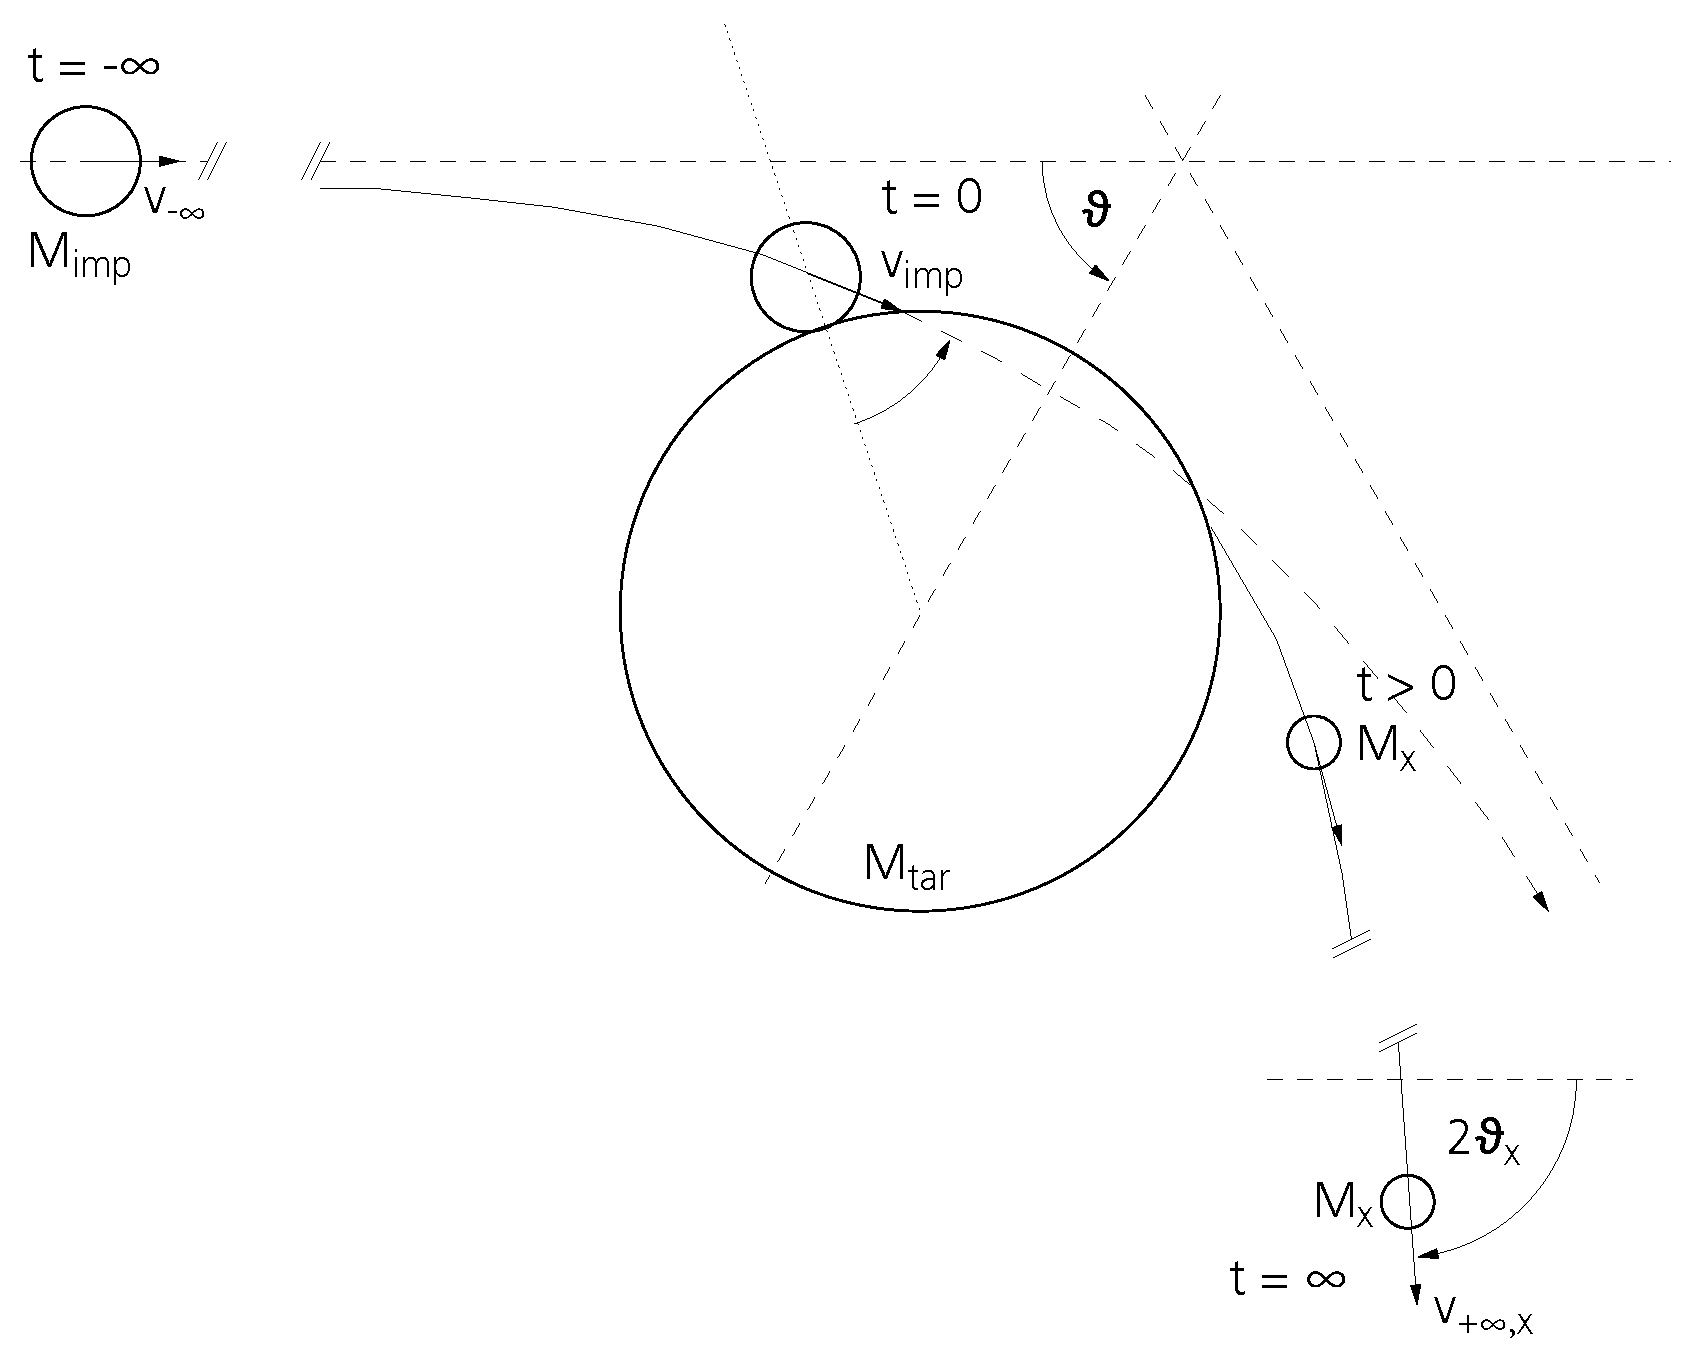
\includegraphics[scale=0.5]{04_vartheta}
\caption{Visualization of the deflection angle: The impactor approaches the target on a hyperbola (or on a parabola in case of $\vinf = 0$). Without a collision the total deflection angle of the impactor would be simply $2 \vartheta$.}
\label{ch03_fig02}
\end{center}
\end{figure}

\begin{landscape}

\begin{figure}[htbp]
\begin{center}
\includegraphics[scale=1.0]{21_SR_vinf_c1.pdf}
\caption{Relative velocity between the largest remnant and the second remnant at infinity as a function of impact angle for the simultion set \emph{c1}. Only simulations are shown, where the second remnant has at least $10\%$ of the mass of the impactor.}
\label{ch03_fig21a}
\end{center}
\end{figure}

\begin{figure}[htbp]
\begin{center}
\includegraphics[scale=1.0]{21_SR_vinf_i1.pdf}
\caption{Relative velocity between the largest remnant and the second remnant at infinity as in figure \ref{ch03_fig21a}, but for simulation set \emph{i1}.}
\label{ch03_fig21b}
\end{center}
\end{figure}

\begin{figure}[htbp]
\begin{center}
\includegraphics[scale=1.0]{22_SR_vartheta_c1.pdf}
\caption{Difference between the actual deflection angle of the second remnant and the expected deflection angle $2 \vartheta_{orb}$ for the impactor assuming an orbit of two point masses as a function of impact angle for simulation set \emph{c1}. Only simulations are shown, where the second remnant has at least $10\%$ of the mass of the impactor.}
\label{ch03_fig22a}
\end{center}
\end{figure}

\begin{figure}[htbp]
\begin{center}
\includegraphics[scale=1.0]{22_SR_vartheta_i1.pdf}
\caption{Difference between the actual deflection angle of the second remnant and the expected deflection angle $2 \vartheta_{orb}$ for the impactor assuming an orbit of two point masses as a function of impact angle for simulation set \emph{i1}. Only simulations are shown, where the second remnant has at least $10\%$ of the mass of the impactor.}
\label{ch03_fig22b}
\end{center}
\end{figure}
\end{landscape}


%%
% ejecta 
%% 
\subsection{Ejecta}
% radiation transfer
Shocks in similar-sized collisions are another departure from 
\begin{align}
\tau_{cool} = \frac{c^2 \sigma}{ 2 \sigma_{SB} T^4}
\end{align}
\cite{Thompson:1988p3451}
radiation transfer: not important because of short timescales (everything in opaque thermal equilibrium): compare stefan boltzmann cooling power (Pahlevan?)


cite Lisse\\
analyze ejecta, entropy and energy of ejecta \\
show decay of shock wave plot\\ % TODOPLOT

\begin{landscape}
\begin{figure}
\begin{center}
\includegraphics[scale=1.0]{20_ejecta_r3.pdf}
\caption{Mass averaged mean disk eccentricities for the largest remnant disk as a function of impact angle for different impact velocities in the \emph{r3} simulation set. Simulations with a largest remnant disk mass below $0.1\% M_tot$ are omitted.}
\label{ch03_fig20a}
\end{center}
\end{figure}

\begin{figure}
\begin{center}
\includegraphics[scale=1.0]{20_ejecta_c1.pdf}
\caption{Mass averaged mean disk eccentricities for the largest remnant disk as a function of impact angle for different impact velocities in the \emph{r3} simulation set. Simulations with a largest remnant disk mass below $0.1\% M_tot$ are omitted.}
\label{ch03_fig20b}
\end{center}
\end{figure}

\begin{figure}
\begin{center}
\includegraphics[scale=1.0]{20_ejecta_i1.pdf}
\caption{Mass averaged mean disk eccentricities for the largest remnant disk as a function of impact angle for different impact velocities in the \emph{r3} simulation set. Simulations with a largest remnant disk mass below $0.1\% M_tot$ are omitted.}
\label{ch03_fig20c}
\end{center}
\end{figure}
\end{landscape}



\section{Discussion}
little toy model population in the early solar system (-> chambers) \\
% TODO: a little estimate for a toy model population in the early solar system: take 4 different sized bodies and analyze collisions into each other. make a plot with transition probabilities?

discuss topics in the light of the results. for example for Moon formation

\begin{figure}[htbp]
\begin{center}
\includegraphics[scale=0.7]{06_vimp}
\caption{An order of magnitude estimation of the random velocities for bodies undergoing collisions in a protoplanetary system with a solar mass central star. The random velocity is roughly the Kepler velocity times the orbital eccentricity. Shown are isolines of velocities for given distance from a star with a solar mass for given eccentricities. The red line shows the speed of sound of for quartz at standard conditions \cite{Melosh:2007p3502}. Note that the actual impact velocity is given by $\vimp = \sqrt{ v_{rand}^2 + \vesc^2}$ and depends on the masses of the two colliding bodies. Due to the high Kepler velocity in the inner parts of the system, even small eccentricities lead to random velocities well above the speed of sound for silicates and therefore to hypervelocity impacts even for small bodies.}
\label{ch03_fig06}
\end{center}
\end{figure}






	
\cite{Agnor:2004p3329}
%Agnor \& Asphaug 2004: accretion efficiency during planetary collisions
%- impact probability of eps: dP = 2*sin(eps)*cos(eps)*deps (Shoemaker 1962)
%- non-disruption doesn't mean merging
%- M1: largest remnant, M2: largest escaping remnant
%- M2 / Mesc < 0.8 for 30deg -> chains
%- two 0.1Mearth mass bodies, chondritic, Tillotson
%- non-accretionary collisions are the norm

\cite{Asphaug:2006p3729}
%Asphaug 2006: h\&r planetary collisions
%- 0deg: shocks dominate, 90deg gravity (tides, stresses) dominates
%- "strings of pearls"
%- for large bodies, the impactor, not the target, are destroyed
%- tidal vs. self-gravity stress inversely proportional to mass
%- relativ energy deposition 

\cite{Asphaug:2010p3539}
%Asphaug 2010: SSC collisions and the diversity of planets
%- next-largest bodies (NLB)
%- hit&run common for v_rand = v_inf
%- Safronov number 1-2 in late systems
%- SSC: contact compression timescale  (2r/v_imp) on gravity timescale ( r*sqrt(G*rho) )
%- shear stress exceeds strength above 100km
%- turn-around the target reference frame: the impactor is the altered body
%- Agnor 1999: angular momentum easily above dynamical stability
%- SSC scale-invariant to the first order
%- 45deg as the median impact angle (Shoemaker 1962)
%- small r/R -> impact cratering
%- "grazing": center of impactor skims tangential to the target
%- impact cratering: angle gives all or nothing, SSC is a continuum
%- for r_core = 0.5*r -> 30deg to 90deg miss each others cores
%- h&r prevalent for NLB
%- NLBs get mantle-stripped
%- tidal disruption important for small bodies
%- icy collision might be similar to rocky ones (ice : rock ~ rock : iron)
%- iron-enriched fragments from chain-events
%- h&r happen to about half the NLB?


\cite{2009ApJ...700L.118M}
%Marcus 2009:
%- confirmation of Stewart & Leinhardt 2009 for bodies > 100km
%- masses 1., 5., 10. Mearth, ratios 0.25, 0.50, 0.75
%- scaling relationship for MFe / Mlr
%- compositional changes require: a) small impact angle or b) small & fast impactor

\cite{2010ApJ...712L..73M}
%Marcus et al. 2010: Minimum radii from Super-Earths: Constraints from GIs
%- super-Mercuries are not expected, as striping bodies would have to be > 10 MEarth

\cite{2010ApJ...714L..21K}
%Kokubo \& Genda 2010:
%- about half the collisions do not accrete
%- orbit integration of 16 bodies, total mass 2.3MEarth
%- mass ratios: 1.0, 0.66, 0.50, 0.33, 0.25, 0.17, 0.11, Mtot = 0.2-2.0MEarth
%- impact velocities: 1.0-3.0 v_esc, angles: 0-75deg
%- criteria for critical impact velocity v_cr / v_esc for which accretion occurs
%- critical spin angular velocity

\cite{2011arXiv1105.4616E}
%Elser et al, 2011:
%- Moon formation in planetary systems
%- might be crucial for life

\cite{Chambers:2001p2105}
\citep{chandrasekhar1969ellipsoidal}
\cite{Lissauer:1993p56}
\cite{Wetherill:1993p3351}


\bibliographystyle{plainnat}
\bibliography{bibliography}



